\chapteropen{Chapter 10: Object design and design patterns}{chapter-10}
\markboth{Ch. 10 | Design patterns}{}

\begin{eli5box}Strategy changes behaviour; Factory creates the chosen object; Observer tells subscribers about changes; Facade offers one simple entry point.\end{eli5box}
\textbf{Answer check:} Name the problem and variation, map roles to the case, show relationships, then give a benefit and cost.
\subsection*{Pattern selection at a glance}


{\fontsize{9}{11}\selectfont
\begin{longtable}{L{.17\linewidth}L{.76\linewidth}}
\toprule\rowcolor{ice}\textbf{Pattern} & \textbf{Use when /\allowbreak{} mechanism /\allowbreak{} cost}\\\midrule\endhead
Strategy & Behaviour/\allowbreak{}algorithm varies; Context delegates to a stable interface. Extra indirection and selection.\\
Factory & Concrete type is known at runtime; centralise creation. Selection/\allowbreak{}configuration still needs maintenance.\\
Observer & Subscribers change over time; attach/\allowbreak{}detach/\allowbreak{}notify through an abstraction. Order, overhead and lifecycle cleanup matter.\\
Fa\c{c}ade & A subsystem is complex; offer one higher-level entry point. Poor/\allowbreak{}excessive facades add rework and overhead.\\\bottomrule
\end{longtable}}

\begin{studycolumns}
\vspace{0pt}

\subsection*{10.1 What object design adds over system design}
\sectionlabel{h-101-what-object-design-adds-over-system-design}
\begin{referenceentries}
\textit{\textbf{System design} / \textbf{Object design}}\par\smallskip
\noindent \textbf{System design:} Architecture, subsystems, layers, styles\par
\noindent \textbf{Object design:} \textbf{Detailed} class diagram, interfaces, patterns\par\smallskip
\noindent \textbf{System design:} Decides \emph{where} responsibility lives\par
\noindent \textbf{Object design:} Decides \emph{how} objects collaborate\par\smallskip
\end{referenceentries}\textbf{Object-design activities:} reuse; interface specification (operations, arguments, types, exceptions); restructuring for design goals; speed/\allowbreak{}memory optimisation.
\subsection*{10.2 Why patterns at all?}
\sectionlabel{h-102-why-patterns-at-all}
A pattern names a reusable response to recurring design forces. Its mechanism and consequences matter more than its name.
\subsection*{10.3 The four elements (L13 definition)}
\sectionlabel{h-103-the-four-elements-l13-definition}
\textbf{Name; problem; solution; consequences.} State when it applies, collaborating roles/\allowbreak{}relationships, and the resulting benefits/\allowbreak{}costs.
\subsection*{10.4 GoF 23 --- grouping (know the buckets)}
\sectionlabel{h-104-gof-23--grouping-know-the-buckets}
\begin{referenceentries}
\textit{\textbf{Category} / \textbf{Patterns}}\par\smallskip
\noindent \textbf{\textbf{Creational (5)}}: Abstract Factory, Builder, \textbf{Factory Method}, Prototype, \textbf{Singleton}\par
\noindent \textbf{\textbf{Structural (7)}}: Adapter, Bridge, Composite, \textbf{Decorator}, \textbf{Fa\c{c}ade}, Flyweight, Proxy\par
\noindent \textbf{\textbf{Behavioural (11)}}: Chain of Responsibility, \textbf{Command}, Interpreter, Iterator, Mediator, Memento, \textbf{Observer}, State, \textbf{Strategy}, Template Method, Visitor\par
\end{referenceentries}\subsection*{10.5 Strategy}
\sectionlabel{h-105-strategy}
\textbf{Strategy:} Context holds the Strategy abstraction and delegates operation(). Concrete strategies implement interchangeable behaviour, selected at runtime. Benefit: independent extension/\allowbreak{}encapsulation. Cost: indirection and a selection decision. The Factory below is optional when Strategy alone suffices.
\end{studycolumns}


\par\smallskip\noindent\begin{minipage}{\linewidth}\centering
\phantomsection\label{shared-pattern}
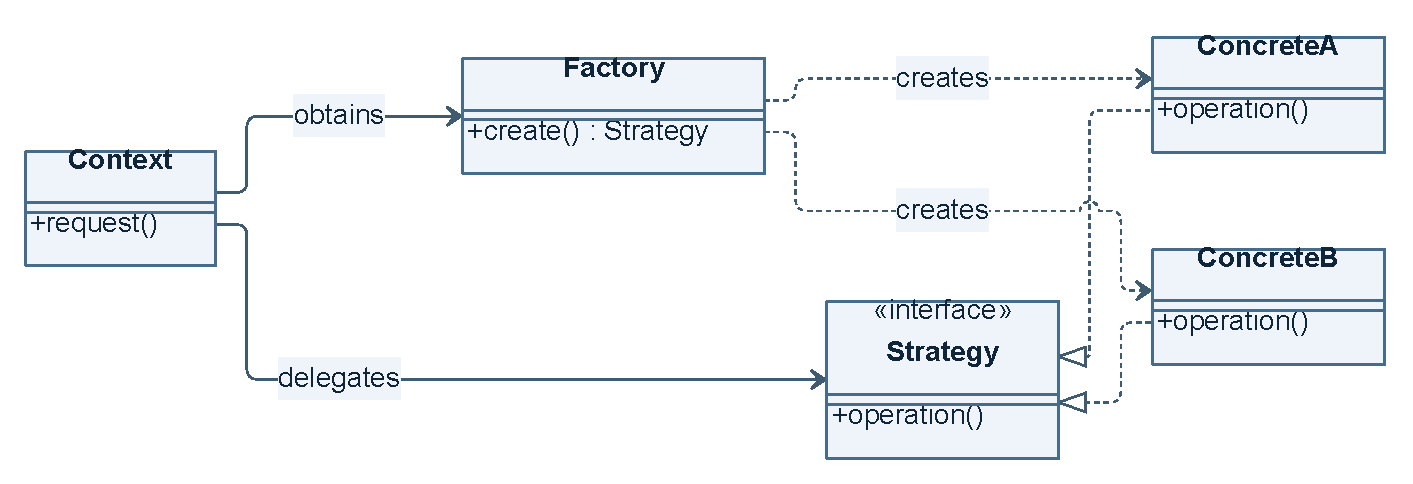
\includegraphics[width=440pt]{images/shared-strategy-factory.pdf}
\captionof{figure}{Canonical Strategy + Factory: substitute the paper's case roles. Factory creates; Context delegates.}\end{minipage}\par\smallskip

\begin{studycolumns}
\vspace{0pt}

\textbf{Template P --- combined-pattern answer:} identify independent behaviour and creation variation; map Context, Strategy, Factory and concrete implementations; show create and delegate relationships; explain extension behind a stable interface plus indirection/\allowbreak{}configuration cost. A switch-based factory still changes for a new type; registration/\allowbreak{}configuration or dynamic loading can move selection out of client code.
\subsection*{10.6 Observer (L13; Tutorial 7)}
\sectionlabel{h-106-observer-l13-tutorial-7}
\textbf{Observer:} Subject holds subscribers through the Observer abstraction; attach/\allowbreak{}detach manage membership, notify calls update. Runtime subscribers and selective interests decouple publisher from concrete listeners; callbacks or messages avoid blind polling. Also called Subscriber--Publisher or Consumer--Producer.
\end{studycolumns}


\par\smallskip\noindent\begin{minipage}{\linewidth}\centering
\begin{minipage}[t]{0.488\linewidth}\centering\scriptsize\textbf{1}\par\smallskip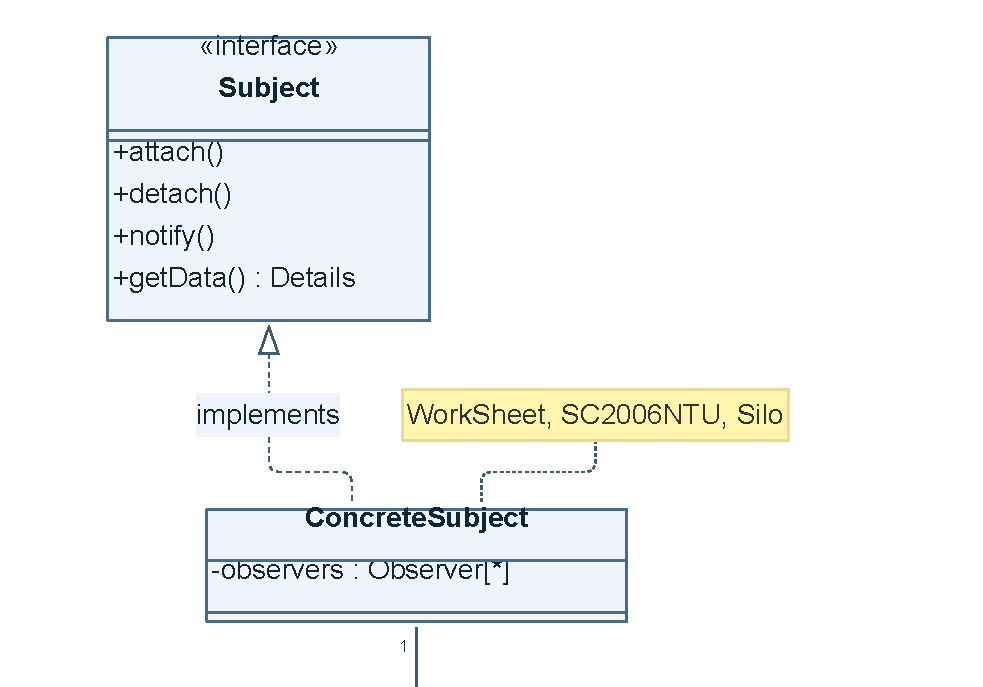
\includegraphics[width=251.00pt]{images/fig-029-compact-1.pdf}\end{minipage}\hfill
\begin{minipage}[t]{0.488\linewidth}\centering\scriptsize\textbf{2}\par\smallskip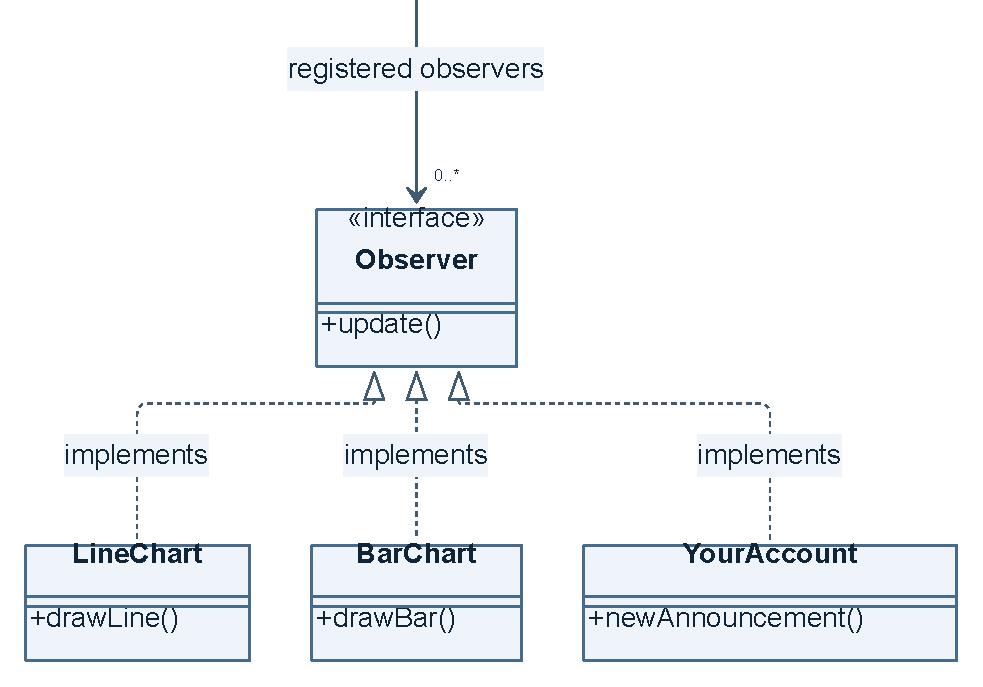
\includegraphics[width=251.00pt]{images/fig-029-compact-2.pdf}\end{minipage}
\captionof{figure}{10.6 Observer (L13; Tutorial 7) --- follow numbered panels; crossing arrows continue.}\end{minipage}\par\smallskip



{\fontsize{9}{11}\selectfont
\begin{longtable}{L{\dimexpr 0.23448\linewidth-5.63pt\relax}L{\dimexpr 0.37198\linewidth-8.93pt\relax}L{\dimexpr 0.39353\linewidth-9.44pt\relax}}
\toprule
\rowcolor{ice}\textbf{} & \textbf{\textbf{Pull}} & \textbf{\textbf{Push}} \\
\midrule\endfirsthead
\toprule\rowcolor{ice}\textbf{} & \textbf{\textbf{Pull}} & \textbf{\textbf{Push}} \\
\midrule\endhead
\multicolumn{3}{r}{\scriptsize Continued on next page}\\\endfoot
\bottomrule\endlastfoot
Subject sends & Simple notification (\code{update()}) & Detailed change data (\code{update(data)}) \\
Observer then & Calls back \code{get\allowbreak{}Data()} --- \textbf{two-way} & Needs no callback --- \textbf{one-way} \\
Coupling & Observer must know the subject's getters & Subject must know what observers need; may over-send \\
Efficiency & Observer fetches only if interested & Wastes data when observer is uninterested \\
\end{longtable}
}

\begin{studycolumns}
\vspace{0pt}
\textbf{Trade-off:} independent reuse and broadcast versus notification overhead, update storms, unspecified order and subscription-cleanup leaks. Selective notification filters registered interests; either push or pull can be used.
\subsection*{10.7 Factory (Static Factory)}
\sectionlabel{h-107-factory-static-factory}
\textbf{Simple/\allowbreak{}Static Factory} centralises runtime selection and construction, removes duplicate creation code and can provide lazy or singleton instances. It differs from GoF Factory Method (subclass-overridden creation) and Abstract Factory (families of related products).

\textbf{Examples:} JDBC creates vendor-specific Connections; Swing selects Look\&Feel; Eclipse loads registered ViewPart subclasses. Dynamic loading supports new configured classes without hard-coding them in the client. Construction remains a separate responsibility from Strategy delegation.
\subsection*{10.8 Fa\c{c}ade}
\sectionlabel{h-108-façade}
\textbf{Fa\c{c}ade} provides a unified higher-level interface to a subsystem. It reduces client dependencies and simplifies use. Costs: a poor facade needs rework; excessive facades add complexity/\allowbreak{}overhead. Direct subsystem access can still exist. Adapter instead converts an incompatible interface.
\end{studycolumns}

\subsection*{10.9 Other patterns you must be able to \emph{name} for a scenario}
\sectionlabel{h-109-other-patterns-you-must-be-able-to-_name_-for-a-scenario}

{\fontsize{9}{11}\selectfont
\begin{longtable}{L{\dimexpr 0.22481\linewidth-5.40pt\relax}L{\dimexpr 0.45466\linewidth-10.91pt\relax}L{\dimexpr 0.32053\linewidth-7.69pt\relax}}
\toprule
\rowcolor{ice}\textbf{Pattern} & \textbf{Scenario signal} & \textbf{Sketch} \\
\midrule\endfirsthead
\toprule\rowcolor{ice}\textbf{Pattern} & \textbf{Scenario signal} & \textbf{Sketch} \\
\midrule\endhead
\multicolumn{3}{r}{\scriptsize Continued on next page}\\\endfoot
\bottomrule\endlastfoot
\textbf{Singleton} & "exactly one instance", configuration/\allowbreak{}registry, lazy init & private ctor, static \code{get\allowbreak{}Instance()} \\
\textbf{Abstract Factory} & "create \textbf{families} of related objects" (controller \emph{or} look-and-feel for a view) & \code{Abstract\allowbreak{}Factory.\allowbreak{}create\allowbreak{}Button()/\allowbreak{}create\allowbreak{}Menu()} \\
\textbf{Factory Method} & Subclasses decide which class to instantiate & \code{creator.\allowbreak{}factory\allowbreak{}Method()} \\
\textbf{DAO} & Isolate persistence from domain logic & \code{Customer\allowbreak{}DAO.\allowbreak{}find(id)} \\
\textbf{Decorator} & Attach \textbf{additional} responsibilities dynamically (e.g. scrolling on a view) & \code{Scrolling\allowbreak{}View wraps View} \\
\textbf{Composite} & Nested views (Panel contains Button; nested Panels) & tree of \code{Component} \\
\textbf{Command} & Undo/\allowbreak{}redo of user actions & \code{Command.\allowbreak{}execute()/\allowbreak{}undo()} \\
\textbf{Adapter} & Convert one interface into another expected by the client & wrapper class \\
\textbf{Proxy} & Surrogate controlling access (remote/\allowbreak{}lazy/\allowbreak{}protection) & same interface as real subject \\
\end{longtable}
}
\par\Needspace{65pt}\phantomsection\label{answer-pattern-cost}
\textbf{Template C --- combine/\allowbreak{}criticise patterns:} combine only for distinct compatible forces; shared classes may play several roles if responsibilities stay clear. Give one concrete benefit and one cost (interfaces, indirection, lifecycle/\allowbreak{}configuration or tests). MVC combines Observer and Strategy; a smaller design can be preferable when variation is absent.
